\documentclass[a4paper, 11pt]{article}
\usepackage{graphicx}
\usepackage{amsmath}
\usepackage[pdftex]{hyperref}
\usepackage{placeins}

% Lengths and indenting
\setlength{\textwidth}{16.5cm}
\setlength{\marginparwidth}{1.5cm}
\setlength{\parindent}{0cm}
\setlength{\parskip}{0.15cm}
\setlength{\textheight}{22cm}
\setlength{\oddsidemargin}{0cm}
\setlength{\evensidemargin}{\oddsidemargin}
\setlength{\topmargin}{0cm}
\setlength{\headheight}{0cm}
\setlength{\headsep}{0cm}

\renewcommand{\familydefault}{\sfdefault}

\newcommand{\TODO}[1]{\textbf{TODO:} #1}

\title{Advanced Systems Lab - Milestone \#2}
\author{Erik Jonsson Thoren - jerik\\}
\date{\today}

\graphicspath{{img/}} % Specifies the directory where pictures are stored


\begin{document}
\maketitle

\section{Method}
\begin{enumerate}
	\item Measure Service Times
	\item Measure 1->1000 clients
	\item Measure 1->10 MW
\end{enumerate}

\section{Model}
\subsection{First Approach}
The first model that was designed was a closed form with limited population, see figure \ref{firstmodel}.

\begin{figure}[ch!]
	\centering
		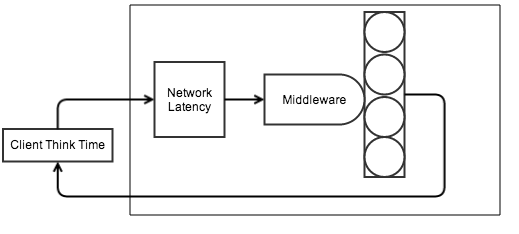
\includegraphics[width=0.8\linewidth]{firstmodel}
		\rule{35em}{0.5pt}
	\caption{Diagram over the first model applied to the system}
	\label{fig:sl1}
\end{figure}


\section{Mean Value Analysis}
Looking at table \TODO{CREATE TABLE OF EXPERMINENTAL DATA FOR THIS} it can be seen that the M/M/1 model for the system is quite accurate according to the MVA.

\begin{table}
    \begin{tabular}{|l|l|l|}
    \hline
    ~          & Experimental & MVA  \\ \hline
    Throughput & 2000         & 1900 \\ \hline
    \end{tabular}
\end{table}
\end{document} 
